%% Преамбула TeX-файла

% 1. Стиль и язык
\documentclass[utf8x]{G7-32} % Стиль (по умолчанию будет 14pt) usepscyr

% Остальные стандартные настройки убраны в preamble.inc.tex.
\sloppy

% Настройки стиля ГОСТ 7-32
% Для начала определяем, хотим мы или нет, чтобы рисунки и таблицы нумеровались в пределах раздела, или нам нужна сквозная нумерация.
\EqInChapter % формулы будут нумероваться в пределах раздела
\TableInChapter % таблицы будут нумероваться в пределах раздела
\PicInChapter % рисунки будут нумероваться в пределах раздела

% Добавляем гипертекстовое оглавление в PDF
\usepackage[
bookmarks=true, colorlinks=true, unicode=true,
urlcolor=black,linkcolor=black, anchorcolor=black,
citecolor=black, menucolor=black, filecolor=black,
]{hyperref}

%\usepackage{pythonhighlight}


\makeatletter
\usepackage{color}
\definecolor{lightgray}{rgb}{0.95, 0.95, 0.95}
\definecolor{darkgray}{rgb}{0.4, 0.4, 0.4}
%\definecolor{purple}{rgb}{0.65, 0.12, 0.82}
\definecolor{editorGray}{rgb}{0.95, 0.95, 0.95}
\definecolor{editorOcher}{rgb}{1, 0.5, 0} % #FF7F00 -> rgb(239, 169, 0)
\definecolor{editorGreen}{rgb}{0, 0.5, 0} % #007C00 -> rgb(0, 124, 0)
\definecolor{orange}{rgb}{1,0.45,0.13}
\definecolor{olive}{rgb}{0.17,0.59,0.20}
\definecolor{brown}{rgb}{0.69,0.31,0.31}
\definecolor{purple}{rgb}{0.38,0.18,0.81}
\definecolor{lightblue}{rgb}{0.1,0.57,0.7}
\definecolor{lightred}{rgb}{1,0.4,0.5}
\usepackage{upquote}
\usepackage{listings}

\lstdefinestyle{py} {%
language=python,
literate=%
*{0}{{{\color{lightred}0}}}1
{1}{{{\color{lightred}1}}}1
{2}{{{\color{lightred}2}}}1
{3}{{{\color{lightred}3}}}1
{4}{{{\color{lightred}4}}}1
{5}{{{\color{lightred}5}}}1
{6}{{{\color{lightred}6}}}1
{7}{{{\color{lightred}7}}}1
{8}{{{\color{lightred}8}}}1
{9}{{{\color{lightred}9}}}1,
basicstyle=\footnotesize\ttfamily, % Standardschrift
numbers=left,               % Ort der Zeilennummern
%numberstyle=\tiny,          % Stil der Zeilennummern
%stepnumber=2,               % Abstand zwischen den Zeilennummern
numbersep=5pt,              % Abstand der Nummern zum Text
tabsize=4,                  % Groesse von Tabs
extendedchars=true,         %
breaklines=true,            % Zeilen werden Umgebrochen
keywordstyle=\color{purple}\bfseries,
frame=b,
commentstyle=\color{brown}\itshape,
stringstyle=\color{editorOcher}\ttfamily, % Farbe der String
showspaces=false,           % Leerzeichen anzeigen ?
showtabs=false,             % Tabs anzeigen ?
xleftmargin=17pt,
framexleftmargin=17pt,
framexrightmargin=5pt,
framexbottommargin=4pt,
%backgroundcolor=\color{lightgray},
showstringspaces=false,      % Leerzeichen in Strings anzeigen ?
}%

\lstdefinestyle{htmlcssjs} {%
  % General design
%  backgroundcolor=\color{editorGray},
  basicstyle={\footnotesize\ttfamily},
  frame=b,
  % line-numbers
  xleftmargin={0.75cm},
  numbers=left,
  stepnumber=1,
  firstnumber=1,
  numberfirstline=true,
  % Code design
  identifierstyle=\color{black},
  keywordstyle=\color{blue}\bfseries,
  ndkeywordstyle=\color{editorGreen}\bfseries,
  stringstyle=\color{editorOcher}\ttfamily,
  commentstyle=\color{brown}\ttfamily,
  % Code
  language=HTML5,
  alsolanguage=JavaScript,
  alsodigit={.:;},
  tabsize=2,
  showtabs=false,
  showspaces=false,
  showstringspaces=false,
  extendedchars=true,
  breaklines=true,
  % German umlauts
  literate=%
  {Ö}{{\"O}}1
  {Ä}{{\"A}}1
  {Ü}{{\"U}}1
  {ß}{{\ss}}1
  {ü}{{\"u}}1
  {ä}{{\"a}}1
  {ö}{{\"o}}1
}

% Изменение начертания шрифта --- после чего выглядит таймсоподобно.
% apt-get install scalable-cyrfonts-tex

\IfFileExists{cyrtimes.sty}
    {
        \usepackage{cyrtimespatched}
    }
    {
        % А если Times нету, то будет CM...
    }

\usepackage{graphicx}   % Пакет для включения рисунков
\DeclareGraphicsExtensions{.jpg,.pdf,.png}
% С такими оно полями оно работает по-умолчанию:
% \RequirePackage[left=20mm,right=10mm,top=20mm,bottom=20mm,headsep=0pt]{geometry}
% Если вас тошнит от поля в 10мм --- увеличивайте до 20-ти, ну и про переплёт не забывайте:
\geometry{right=20mm}
\geometry{left=30mm}

\usepackage{subfig}

% Произвольная нумерация списков.
\usepackage{enumerate}

\usepackage{amsmath}

\onehalfspacing

\setcounter{tocdepth}{1} %Подробность оглавления
%4 это chapter, section, subsection, subsubsection и paragraph
%3 это chapter, section, subsection и subsubsection
%2 это chapter, section, и subsection
%1 это chapter и section
%0 это chapter.


\begin{document}

\begin{center}
    Министерство образования и науки Российской Федерации\\
    Федеральное государственное автономное образовательное учреждение высшего профессионального образования\\
    «Московский физико-технический институт \pt(государственный~университет)»\\[10mm]

    Факультет проблем физики и энергетики\\[5mm]
    Кафедра физики высоких плотностей и энергий\\[15mm]

    \textbf{
        СПЕКТРАЛЬНАЯ ДИАГНОСТИКА ПЫЛЕВОЙ ПЛАЗМЫ В ГАЗОВОМ РАЗРЯДЕ ПОСТОЯННОГО ТОКА\\[10mm]
    }

    Выпускная квалификационная работа\\
    (магистерская диссертация)\\[5mm]

Направление подготовки: 03.04.01 Прикладные математика и физика\\[15mm]
\end{center}
Выполнил:\\
студент 282 группы \uline{\hfill} Шоненков Алексей Владимирович\\[10mm]
Научный руководитель:\\
к.ф.-м.н. \uline{\hfill} Усачев Александр Дмитриевич\\[10mm]
%Научный консультант:\\
%к.ф.-м.н.  \uline{\hfill} Зобнин Андрей Вячеславович
\vfill

\begin{center}
    Москва, 2018
\end{center}

\thispagestyle{empty}


\frontmatter % выключает нумерацию ВСЕГО; здесь начинаются ненумерованные главы: реферат, введение, глоссарий, сокращения и прочее.

\chapter*{Аннотация}

В данном исследовании разработан метод измерения относительного изменения температуры электронов $T_e$
в стационарном однородном положительном столбе слаботочного газового разряда
постоянного тока в неоне низкого давления под влиянием протяженного пылевого
облака в космических условиях по изменению интенсивности различных спектральных линий.
Был проведен эксперимент, с помощью которого получена оценка согласованности с разработанным подходом.
Впервые на основе эмиссионных спектров было расчитано абсолютное значение электронной температуры $T_e$ и осевого
электрического поля $E_z$ возмущенного пылевым облаком газового разряда, используя параметры невозмущенного разряда.
Невозмущенный разряд: $E_z = 2.2$~В/см, $T_e = 3.2$~В/см.
Возмущенный разряд: $E_z = 2.8$~В/см, $T_e = 3.5$~В/см.

В ходе данной работы был создан веб-сервис «Spectral~Analyzer~PK-4», который позволяет обрабатывать
спектральные данные экспериментов, проведенных на научной аппаратуре «Плазменный~кристалл~-~4». Данный веб-сервис
уникален и также имеет свой научный вклад в мировое сообщество.

\vfill
\vfill
\begin{minipage}{.49\textwidth}\end{minipage}
\hfill
\begin{minipage}{.49\textwidth}
    Автор: \uline{\hfill} Шоненков А.В.
\end{minipage}
\vfill


\setcounter{page}{3}

\tableofcontents

\clearpage

\Introduction

Диагностика плазмы является основой для выбора теоретических моделей и интерпретации полученных данных.
Главные диагностируемые параметры в не намагниченной плазме - концентрация ионов \math{n_i}$
и электронов \math{n_e}$, температура ионов \math{T_i}$ и электронов \math{T_e}$,
функция распределения электронов \math{f_e}$, а также распределение
пространственно-электрического потенциала \phi(r)$. Зная последнее, можно получить распределение напряженностей
электрических полей \math{E = \phi(r)}$.

Существует целый спектр различных методов диагностики плазмы - электрические (зондовые), оптические, спектральные,
корпускулярные, микроволновые [?...ССЫЛКА НА ИСТОЧНИК...?]. Как правило, плазма существенно неоднородная, а измерения содержат
существенные ошибки. Наиболее достоверными являются параметры плазмы, измеренные двумя независимыми методами.
Использование комбинаций различных методов позволяют получать данные, недоступные каждому методу в отдельности.
Например, спектральные методы позволяют экстраполировать в пространстве данные зондовых измерений.

Несмотря на свой почтенный возраст, зондовая диагностика остается наиболее достоверным базовым видом диагностики плазмы.
В общем случае из полученной зондовой вольт-амперной характеристики можно извлечь все основные параметры плазмы.
Основным недостатком зондового метода является его инвазивность и необходимость обустройства специальных фланцев для ввода зондов.
Что касается зондовой диагностики пылевой плазмы, то она мало перспективна ввиду того, что зонд крайне сильно возмущает пылевое облако.
В настоящее время на Международной космической станции (МКС) находится российско-европейская научная аппаратура
«Плазменный~кристалл~-~4» (НА~«ПК-4») для изучения фундаментальных свойств пылевой плазмы в положительном столбе
газового разряда низкого давления. Одной из задач этого эксперимента является изучение влияния пылевой компоненты
на спектр излучения положительного столба и определение по этому изменению спектра изменение параметров плазмы -
в первую очередь изменения электронной температуры. Полноценная интерпретация полученных спектральных данных требует
составления и самосогласованного решения кинетического уравнения Больцмана в нелокальном приближении для положительного
столба с пылевой компонентой, что является сложной задачей.

Целью данной работы является исследование влияния протяженного пылевого облака на спектральные характеристики
положительного столба газового разряда и определение по данным характеристикам изменения электронной температуры
в облаке.

В связи с этим, был проведен обзор экспериментальных спектральных данных, полученных на научной аппаратуре «ПК-4» за
время ее эксплуатации, выбор наиболее удачных с точки зрения поставленной задачи экспериментов, обработка спектров
и их интерпретация в рамках столкновительно-радиационной модели.


\mainmatter

\chapter{Спектральная диагностика~низкотемпературной плазмы газового разряда}
%\chapter{СПЕКТРАЛЬНАЯ ДИАГНОСТИКА НИЗКОТЕМПЕРАТУРНОЙ ПЛАЗМЫ ГАЗОВОГО РАЗРЯДА}
\label{cha:ch_1}
\section{Кинетика заселения возбужденных атомных состояний в плазме}
Спектры излучения газоразрядной плазмы определяются населенностью \math{N_j}$ соответствующих возбужденных атомных уровней \math{E_j}$.
Тогда интенсивность соответствующей атомной спектральной линии составит:
\begin{equation}
    I_{ji} = A_{ji}h\nu_{ji}⋅N_j
\end{equation}
где \math{A_{ji}}$  - коэффициент Эйнштейна для перехода \math{j → i}$, \math{N_j}$ - населенность возбужденного уровня \math{j}$.

Таким образом, задача спектральной диагностики плазмы сводится к построению теоретических моделей, связывающих
параметры плазмы (в первую очередь, концентрации электронов \math{n_e}$ и их температуру \math{T_e}$) с интенсивностями спектральных
линий \math{I_{ji}}$. Выбор той или иной модели зависит от параметров плазмы: ее химического состава, плотности,
степени ионизации и равновесности. В данной работе экспериментально и теоретически исследуется стационарная сильно
неравновесная плазма положительного столба слаботочного газового разряда постоянного тока (\math{I_{DC}~=~1}$~мА)
в неоне при давлении \math{P~=~60}$~Па, причем степень ионизации плазмы α очень мала (\math{\alpha~\sim~10^{-8}}$).
Выбор этих параметров обуславливается практическим случаем, рассматриваемым в этой работе.
\begin{figure}[t]
    \begin{center}
         \subfloat[\label{sub:fig11a}]{
           \includegraphics[width=0.35\textwidth]{figures/fig11a}
         }
         \hspace{0.05\columnwidth}
         \subfloat[\label{sub:fig11b}]{
           \includegraphics[width=0.305\textwidth]{figures/fig11b}
         }
         \caption{Схема основных процессов уровня: \pt(a) заселение, \pt(b) расселение.}
         \label{fig:fig11}
    \end{center}
\end{figure}

Населенность \math{N_j}$ уровня \math{E_j}$ в стационарном случае определяется балансом процессов его заселения
и расселения. Схема основных процессов заселения уровня \math{E_j}$ представлена на рис.~\ref{fig:fig11}~\subref{sub:fig11a}.
Основным процессом заселения рассматриваемого уровня \math{E_j}$ является его заселение прямым
электронным переходом с основного состояния \math{E_0}$ и с метастабильного \math{E_i}$.

Скорости процессов \math{C_{0j}}$ и \math{C_{ij}}$ определяются соотношениями:
\begin{equation}C_{0j} = \sqrt{2 \over m_e} \int_{E_j}^{\infty} \sigma_{0j}(E) f_e(E) \sqrt{E} dE\end{equation}
и
\begin{equation}C_{ij} = \sqrt{2 \over m_e} \int_{E_j - E_i}^{\infty} \sigma_{ij}(E) f_e(E) \sqrt{E} dE\end{equation}
соответственно, где …

Сечения \math{\sigma_{0j}(E)}$ и \math{\sigma_{ij}(E)}$ расчетные и экспериментальные, можно найти в литературе
или базе данных NIST [ССЫЛКА НА ИСТОЧНИК]. Типичный вид сечений представлен на рис. \ref{fig:fig12}.
Что касается вида ФРЭ, то она сильно зависит от параметров плазмы. При высоких давлениях ФРЭ приближается
к максвелловской функции. Однако, при низких давлениях плазма сильно неравновесна, и вид функции ФРЭ должен
быть определен дополнительными методами. Кроме столкновительного заселения уровень \math{E_j}$ заселяется
также путем радиационного распада верхних \math{k}$-уровней \math{E_k~>~E_j}$ cо скоростью \math{A_{kj}}$ при \math{k > j}$.
Значения \math{A_{kj}}$ также табулированы в базе данных NIST.
\begin{figure}[t]
  \centering
  \includegraphics[width=8cm]{figures/fig12}
  \caption{Типичный вид сечения \math{\sigma}$ и максвелловской ФРЭ. \math{T_e}$ - температура электронов, \math{E_{thr}}$ - пороговая энергия..}
  \label{fig:fig12}
\end{figure}

Схема основных процессов расселения уровня \math{E_j}$ представлена на рис.~\ref{fig:fig11}~\subref{sub:fig11b}.
Этими процессами также являются явления спонтанного распада возбужденных уровней и столкновительные процессы,
индуцированные свободными электронами.

Приравняв скорости заселения и расселения уровня \math{E_j}$, мы получим уравнение относительно ФРЭ \math{f_e(E)}$.
Это уравнение является некорректной задачей и для ее решения необходимы дополнительные данные о виде ФРЭ.
Эти данные могут быть получены путем решения кинетического уравнения Больцмана для соответствующих условий.

\section{Уравнение Больцмана для ФРЭ в положительном столбе газового разряда постоянного тока.}

Газовые разряды представляют собой крайне неравновесную систему, в которой средняя энергия электронов (температура)
на два порядка превышает температуру газа. Функция распределения электронов (ФРЭ) характеризуется нагревом
электронов электромагнитными полями и столкновениями их с нейтральными атомами, почти во всех случаях это распределение
отклоняется от равновесного (Максвелловского). Решение кинетического уравнения Больцмана для ФРЭ является
важнейшей задачей для точного моделирования плазмы, так как многие явления невозможно правильно понять
без кинетического анализа. Уравнение Больцмана существенно можно упростить из-за большого различия масс электронов и атомов.
В силу данного различия, затухание энергии электронов в упругих столкновениях с атомами происходит гораздо медленнее,
чем затухание импульса электронов (\math{m_e \ll M_a}$). Как следствие, ФРЭ в скоростном пространстве может быть представлена как сумма
большой изотропной \math{f_0}$ и малой анизотропной частей \math{f_1}$.

Выделяют три существенно различных случая. Первый случай, когда величины \math{P L \gg 1}$ и \math{{E P} \ll 1}$, где
\math{P}$ - давление газа, \math{L}$ - характерный размер плазмы, \math{E}$ - электрическое поле, а
пространственные градиенты \math{f_0}$ и \math{f_1}$ малы и определены локальными значениями электрического поля,
электронной плотности и составом плазмы. Тогда электроны могут быть описаны уравнениями жидкости с коэффициентами переноса,
полученными из локальной (не Максвелловской) ФРЭ. Обычно через уравнение Больцмана решают задачу нахождения
коэффициентов переноса и скоростей протекания реакции для данного приближения.

Второй случай соответствует столкновительной плазме, где характерный размер плазмы \math{L}$ значительно больше средней длины
свободного пробега электронов \math{\lambda}$, но сравним с длиной релаксации энергии электрона \math{\lambda_\epsilon}$.
В этом нелокальном режиме изотропная часть ФРЭ \math{f_0}$ в заданной точке зависит не только от электрических полей в этой точке,
но и от свойств плазмы в окрестности точки размера (эффект памяти), а анизотропная часть \math{f_1}$ является лишь функцией
электрического поля \math{E}$. В этом столкновительном режиме плазма не может быть описана гидродинамикой.

В третьем случае, при дальнейшем уменьшении \math{P L}$, средняя длина свободного пробега электрона будет сравнима c характерным размером плазмы
(\math{\lambda \sim L)$. В этом почти бесстолкновительном случае анизотропная часть в точке определяется не только
значением напряженности электрического поля в этой точке, но и профилем электрического поля вдоль траектории электрона.
В результате локальная зависимость между плотностью тока и электрическим полем (закон Ома) становится недействительной \cite{Kolobov}.

Плазма тлеющего разряда низкого давления имеет сильно неравновесный характер. Рождение заряженных частиц происходит
преимущественно в объемных процессах, а гибель на стенках разрядной камеры. Энергию электроны приобретают,
разгоняясь в электрическом поле, а теряют в упругих и неупругих столкновениях. Количественное описание этих процессов
возможно только на кинетическом уровне \cite{Zobnin}.

В данной работе положительный столб газового разряда находится под низким давлением порядка 60~Па и имеет диаметр трубки 30~мм (см. раздел \ref{sec:sec_31}),
а значит для описания кинетических процессов с помощью уравнения Больцмана необходимо пользоваться почти бесстолкновительным приближением.

Кинетическое уравнение Больцмана представляет собой интегродифференциальное уравнение, описывающее эволюцию функции
распределения частиц в шестимерном (6-D) фазовом пространстве. Данное уравнение было выведено Людвигом Больцманом в 1872 г.
Оно до сих пор остается основой кинетической теории газов и оказывается плодотворным не только для исследования
классических газов, которые имел в виду Больцман, но - при соответствующем обращении - и для излучения переноса
электронов в твердых телах и плазме \cite{Cherchin'yani}. В общем виде оно выглядит следующим образом (также данное
уравнение называют уравнением Власова):

\begin{equation}
    {\partial f_e \over \partial t} + (\vec{v}, \vec{\Delta}_r) f_e + (\vec{a}, \vec{\Delta}_v) f_e = I
    \label{eq:vlasov}
\end{equation}
где \math{f_e = f_e(\vec{r}, \vec{v}, t)}$~--~функция распределения электронов,
\math{\vec{r}}$~--~вектор положения в физическом пространстве, \math{\vec{v}}$~--~вектор скорости,
\math{\vec{a}}$~--~вектор ускорения, \math{t}$~--~время, \math{I}$~--~интеграл столкновений,
является интегральным оператором в пространстве скоростей, в котором должны быть учтены все элементарные процессы
с участием электронов, приводящие к изменению их числа в объеме \math{dx dy dz dv_x dv_y dv_z}$ фазового пространства.

Решение этого интегродифференциального нелинейного уравнения сопряжено с огромными математическими трудностями и
поэтому всегда проводится с привлечением ряда серьезных упрощений. Многие сотни журнальных публикаций посвящены
конкретным расчетам \math{f(V)}$ в различных условиях, однако среди них далеко не всегда удается найти требуемое.
Вместе с тем экспериментатору часто приходится хотя бы оценить ожидаемый вид \math{f(V)}$ в условиях его работы \cite{Kolesnikov}.

%{e \over m_e} \vec{E}

Для слабоионизированной плазмы столкновения электронов с нейтралами обычно преобладают над столкновениями между
заряженными частицами. Из-за разницы масс электрона и атома (\math{m_e \ll M_a}$) интеграл столкновения
для упругих взаимодействий электронов с тяжелыми нейтралами может быть записан в так называемой форме Лоренцевского газа
\cite{Kolobov}:
\begin{equation}
    I_{el} = - {1 \over v^2} {\partial \over \partial v} v^2 \Gamma - N v \int_{S^2} \sigma (v, |\Omega - \Omega^{'}|) [f(v, \Omega^{'}) - f(v, \Omega)] d \Omega
    \label{eq:lorentz}
\end{equation}
где \math{\Omega}$~--~телесный угол фазового пространства скоростей на единичной сфере \math{S^2}$ (\math{\vec{v} = v \Omega}$),
\math{\sigma}$~--~сечение столкновения, \math{N}$~--~концентрация атомов газа, поток \math{\Gamma}$ задается следующим образом:
\begin{equation}
    \Gamma = - {\delta \nu \over 2} \big{(} v f + {T \over m} {\partial f \over \partial v} \big{)}
\end{equation}
где \math{T}$~--~температура газа, \math{\nu}$~--~транспортная частота столкновений и \math{\delta = (2m / M)}$~--~
средняя доля энергии, которая теряется электронами в упругих столкновений. Первое слагаемое в (\ref{eq:lorentz}) мало, оно
отвечает за обмен энергиями между электронами и нейтралами. Второе слагаемое в (\ref{eq:lorentz}) описывает столкновения
электронов с бесконечно тяжелыми частицами, которые в основном не меняют свою энергию, а лишь изотропно меняют
распределение электронов. Таким образом для того, чтобы ФРЭ пришла в равновесие с полем необходимо, чтобы прошло время
намного превышающе \math{({\nu m / M})^{-1}}$ \cite{Tsendin}.

Таким образом, для почти бесстолкновительного случая в качестве приближения ФРЭ для решения уравнения Власова (\ref{eq:vlasov}) можно
использовать достаточно распространенное двухчленное приближение:
\begin{equation}f_e(\vec{r}, \vec{v}, t) = f_0(\vec{r}, \vec{v}, t) + { \vec{v} \over v} \vec{f_1} (\vec{r}, \vec{v}, t)\end{equation}
где \math{f_1}$ отвечает за анизотропию.

Подставив это приближение в уравнение (\ref{eq:vlasov}) и усреднив по направлениям скоростей (в силу их изотропности из-за
столкновений с тяжелыми частицами), получим следующую систему уравнений, которую называют системой
Давыдова-Эллиса \cite{Kolobov}:
\begin{equation}
 \begin{cases}
  {\partial \vec{f_1} \over \partial t} + \nu \vec{f_1} = - v \nabla f_0 - {e \vec{E} \over m} {\partial f_0 \over \partial v},
   \\
   {\partial f_0 \over \partial t} + {v \over 3} div(\vec{f_1}) + {1 \over 3v^2} {\partial \over \partial v } ({ v^2 e \vec{E} \over m} \vec{f_1} ) = S_0
 \end{cases}
 \label{eq:davydov-ellis}
\end{equation}
Здесь \math{e}$~--~модуль заряда электрона, \math{m}$~--~масса электрона, \math{S_0}$ —  часть интеграла столкновений,
отвечающая за упругие и неупругие электрон-атомные столкновения и электрон-электронные взаимодействия

В левой части первого уравнения системы (\ref{eq:davydov-ellis}) можно пренебречь слагаемым
{\partial \vec{f_1} \over \partial t}$, так как мы рассматриваем выход ФРЭ на стационарный уровень во времени,
где анизотропические эффекты уже не имеют значения.

Перейдя от скоростей к энергиям \math{v = \sqrt{2 \epsilon \over m}}$,
\math{{\partial f(v) \over \partial v}  = {\partial f(\epsilon) \over \partial \epsilon} \sqrt{2 \epsilon m}}$
в системе Давыдова-Эллиса (\ref{eq:davydov-ellis}) и подставив выражение для \math{\vec{f_1}}$ в нижнее уравнение, получим:
\begin{equation}
    \begin{gathered}
        \sqrt{\epsilon} {\partial f_0 \over \partial t} = \sqrt{2 \over m} \big{[} S_0 + {\partial \over \partial \epsilon}
        [\epsilon^{3 \over 2} ({2 m \over M} \nu f_0 + {e^2 (\vec{E}, \vec{E}) \over 3 \nu} {\partial f_0 \over \partial \epsilon})] \big{]}
    \end{gathered}
\end{equation}
где \math{M}$ - масса молекулы неона.

Поскольку столб газового разряда геометрически представляет собой продольную трубку,
вдоль которой течет ток, то модуль электрического поля равен продольной составляющей \math{|\vec{E}|} = E_z}$, также его
называют осевым электрическим полем. Подставив значение транспортной частоты \math{\nu = N_g \sigma_t \sqrt{\epsilon}}$ и
осевого электрического поля, а также выполнив незначительные преобразования (в том числе переобозначение \math{f_0 = f}$), получим:
\begin{equation}
    \begin{gathered}
        \sqrt{\epsilon} {\partial f \over \partial t } = \sqrt{2 \over m} \big{[} S_0 + 2 {m \over M} N_g
        {\partial \over \partial \epsilon} \big{[} \sigma_t \epsilon^2 f \big{]}
        + {e^2 E_z^2 \over 3 N_g} {\partial \over \partial \epsilon} \big{[} {\epsilon \over \sigma_t}
        {\partial f \over \partial \epsilon} \big{]} \big{]}
    \end{gathered}
    \label{eq:main_eq}
\end{equation}

Вид \math{S_0}$ зависит от того, какие взаимодействия с электронами учитываются.
В данной работе использовался следующий вид \math{S_0}$, записанный в дискретной форме:
\begin{equation}
    S_0 = \sum_k \big{[} \sqrt{\epsilon + \epsilon_k} \nu_k (\epsilon + \epsilon_k)f(\epsilon + \epsilon_k) - \sqrt{\epsilon} \nu_k(\epsilon)f(\epsilon) \big{]}
    \label{eq:S_0}
\end{equation}
суммирование проводится по всем верхним энергетическим уровням k, которые больше аргумента функции \math{\epsilon}$,
частота столкновения k-уровня записывается так \math{\nu_k(\epsilon) = \sigma_k(\epsilon)N_g\sqrt{\epsilon}}$,
\math{N_g}$ - концентрация атомов.

В почти бесстолкновительном случае для поиска концентрации атомов Ne \math{N_g}$ можно воспользоваться уравнением состояния идеального газа,
поскольку атомы между собой почти не взаимодействуют:
\begin{equation}
    N_g = {P \over k_b T}
    \label{eq:concentration}
\end{equation}
где \math{P}$~--~давление газа 60~Па; \math{k_b}$~--~постоянная Больцмана; \math{T}$~--~температура газа 294~K.

\section{Решение уравнения Больцмана и результаты}

В данном подразделе описываются численные подходы, алгоритмы и аппроксимации необходимые для нахождения численного решения
функций распределения электронов для различных осевых электрических полей в диапазоне \math{1 \le E_z \le 10}$~В/см,
которые задаются параметрически.

Рассматривается задача решения разностной схемы относительно \math{f}$ на основе уравнений (\ref{eq:main_eq}) и (\ref{eq:S_0}).
Данная задача является краевой: вероятность нахождения электронов при бесконечно большой энергии стремится к нулю, а
вероятность нахождения электронов с положительном энергией максимальна, т.е. первая производная ФРЭ по энергии в нуле
будет равна нулю. Имеем следующие граничные условия:
\begin{equation}
    \begin{cases}
        {d f \over d \epsilon}(0) = 0
        \\
        f(\infty) = 0
    \end{cases}
    \label{eq:borders}
\end{equation}

Если обратить внимание на уравнения (\ref{eq:main_eq}) и (\ref{eq:S_0}), то становится ясно, что аналитически выразить
\math{f}$ для явного построения разностной схемы невозможно, поскольку в (\ref{eq:S_0}) \math{f}$ принимает значения для
аргументов, отличных от \math{\epsilon}$. Следовательно, при данной трактовки задачи необходимо получить дополнительное граничное
условие для каждого элемента суммирования \math{\epsilon_k}$, например с помощью двухточечной краевой задачи (метод стрельбы),
и сводить исходную задачу к задаче Коши. Это довольно сложный подход, более того, нет необходимости для каждого момента времени
решать задачу Коши, поскольку нас интересует ФРЭ при выходе на стационарный уровень во времени, а не при сложных переходных процессах.

Предполагается, что функция распределения электронов при заданном электрическом поле выйдет на стационарый уровень: из-за
невысоких полей данное предположение более, чем разумно. Поэтому будем высчитывать с помощью метода временной эволюции
относительную разницу ФРЭ между итерациями по времени и смотреть, если относительное изменение достаточно незначительно, то ФРЭ вышла
на стационарный уровень; далее решается краевая задача с граничными условиями (\ref{eq:borders}).
Построим разностную схему для данного подхода:
\begin{equation}
\begin{small}
    \begin{gathered}
        f^n(\epsilon) = f^{n-1}(\epsilon) + \Delta t \sqrt{2 \over m \cdot \epsilon}
        \Big{[} N_g \sum_k
            \big{[}
                F^{n-1}_k (\epsilon + \epsilon_k) - F^{n-1}_k (\epsilon)
            \big{]} + \\
        {2 m N_g \over M}
            \big{[}
                {F^{n-1}_t(\epsilon + \Delta \epsilon) \cdot (\epsilon + \Delta \epsilon) -
                F^{n-1}_t(\epsilon - \Delta \epsilon) \cdot (\epsilon - \Delta \epsilon)  \over 2 \Delta \epsilon }
            \big{]} + \\
        {1 \over \Delta \epsilon} \cdot {e^2 E_z^2 \over 3 N_g} \cdot
            \big{[}
                {\epsilon + { \Delta \epsilon \over 2 } \over  \sigma_t(\epsilon + { \Delta \epsilon \over 2 })} \cdot
                {f^{n-1}(\epsilon + \Delta \epsilon) - f^{n-1}(\epsilon) \over \Delta \epsilon } -
                {\epsilon - { \Delta \epsilon \over 2 } \over  \sigma_t(\epsilon - { \Delta \epsilon \over 2 })} \cdot
                {f^{n-1}(\epsilon) - f^{n-1}(\epsilon - \Delta \epsilon) \over \Delta \epsilon }
            \big{]}
        \Big{]}
    \end{gathered}
\end{small}
\label{eq:razh_scheme}
\end{equation}
где \math{\epsilon}$~--~энергия в~эВ; \math{\Delta \epsilon}$~--~шаг по энергии в~эВ;
\math{f^n (\epsilon)}$~--~ФРЭ с энергией \math{\epsilon}$, имеющая \math{n}$-й шаг по времени;
\math{\sigma_t (\epsilon)}$~--~транспортное сечение упругого рассеяния;
\math{\sigma_k (\epsilon)}$~--~сечение неупругих столкновений для k-уровня;
\math{N_g}$~--~концентрация атомов \math{Ne}$ в см^{-3}; \math{M}$~--~масса молекулы Ne в граммах;
\math{m}$~--~масса электрона в граммах; \math{e}$~--~заряд электрона в Кл;
\math{k}$~--~итератор суммирования по всем энергиям верхних уровней, значения которых больше \math{\epsilon}$;
\math{E_z}$~--~осевое электрическое поле, которое задается параметрически в диапазоне \math{1 \le E_z \le 10}$~В/см с шагом \math{0.1}$~В/см;
для удобства записи выполнена замена
\math{F^n_i}(\epsilon) = f^n(\epsilon) \cdot \sigma_i(\epsilon) \cdot \epsilon }$, где \math{i}$ обозначает природу сечения.

На языке разностной схемы граничные условия (\ref{eq:borders}) будут выглядить следующим образом:
\begin{equation}
    \begin{cases}
        f^n_0 = f^n_1
        \\
        f^{n}_K = 0
    \end{cases}
    \label{eq:razn_borders}
\end{equation}
где K~--~максимальное количество шагов по энергии, в рамках данной задачи энергию равной 50~эВ можно считать уже бесконечно большой.
То есть при шаге \math{\Delta \epsilon = 0.1}$~эВ максимальное количество шагов по энергии будет \math{K = 500}$.

В качестве начальных условий при \math{t = 0}$ для первого вычисления ФРЭ (при \math{E = 1}$~В/см) предлагается взять
распределение Больцмана:
\begin{equation}
    f^0 (\epsilon) = 0.7 \cdot e^{- {\epsilon \over 6}}
    \label{eq:start_condition}
\end{equation}

Данная функция намного ближе к итоговому решению, чем прямая, а значит для сходимости нужно будет выполнить меньше итераций
по времени: чем приближеннее возьмем начальное условие, тем быстрее наступит стационарный уровень. По данным соображениям
для подсчета ФРЭ для следующих полей удобнее всего брать за начальные условия результаты предыдущего расчета.

В данной работе использовались следующие аналитические аппроксимации для сечений элементарных процессов, полученные частично из
\cite{Zobnin}, частично из последних трудов Зобнина~А.~В.:
\begin{equation*}
    \sigma_t(\epsilon) = \begin{cases}
    \big{[}
        2.56 + 0.57 \cdot \ln
        \big{(}
            0.02 + {\epsilon \over 5.5 + \epsilon^2 } + {0.15 \cdot \epsilon^2 \over 12 + \epsilon + 3 \cdot 10^{-5} \cdot \epsilon^4}
        \big{)}
    \big{]} \cdot 10^{-16}, \epsilon > 0 \\
    \big{[}2.56 + 0.57 \cdot \ln(0.02)\big{]} \cdot 10^{-16}, \epsilon \le 0
    \end{cases}
\end{equation}
\begin{figure}[t]
  \centering
  \includegraphics[width=15cm]{figures/fig13}
  \caption{Графическое представление некоторых аппроксимаций сечений рассеяния для различных энергетических уровней.}
  \label{fig:fig13}
\end{figure}
\begin{equation*}
    \sigma_{16.62}(\epsilon) = \begin{cases}
    {2.742 \cdot 10^{-14} \over \epsilon^3} \cdot \sqrt{\epsilon - 16.6 \over \epsilon}, \epsilon > 16.62 \\
    0, \epsilon \le 16.62
    \end{cases}
\end{equation}
\begin{equation*}
    \sigma_{16.67}(\epsilon) = \begin{cases}
    {5.01 \cdot 10^{-17} \over \epsilon} \cdot \sqrt{\epsilon - 16.67 \over \epsilon}, \epsilon > 16.67 \\
    0, \epsilon \le 16.67
    \end{cases}
\end{equation}
\begin{equation*}
    \sigma_{16.72}(\epsilon) = \begin{cases}
    {5.941 \cdot 10^{-15} \over \epsilon^3} \cdot \sqrt{\epsilon - 16.7 \over \epsilon}, \epsilon > 16.72 \\
    0, \epsilon \le 16.72
    \end{cases}
\end{equation}
\begin{equation*}
    \sigma_{16.85}(\epsilon) = \begin{cases}
    6 \cdot 10^{-18} \cdot \ln\big{(}{\epsilon \over 16.8}\big{)} + 5.7 \cdot 10^{-18} \sqrt{\epsilon - 16.8 \over \epsilon}, \epsilon > 16.85 \\
    0, \epsilon \le 16.85
    \end{cases}
\end{equation}
\begin{equation*}
    \sigma_{18.38}(\epsilon) = \begin{cases}
    {2.024 \cdot 10^{-17} \over \epsilon + 11} \cdot \sqrt{\epsilon - 18.38 \over \epsilon}, \epsilon > 18.38 \\
    0, \epsilon \le 18.38
    \end{cases}
\end{equation}
\begin{equation*}
    \sigma_{18.6}(\epsilon) = \begin{cases}
    {1.44 \cdot 10^{-16} + 1.4 \cdot 10^{-18} \cdot \epsilon \over \epsilon + 50} \cdot \sqrt{\epsilon - 18.6 \over \epsilon}, \epsilon > 18.6 \\
    0, \epsilon \le 18.6
    \end{cases}
\end{equation}
\begin{equation*}
    \sigma_{18.71}(\epsilon) = \begin{cases}
    {3.461 \cdot 10^{-15} + 1.565 \cdot 10^{-16} \cdot \epsilon + 1.5 \cdot 10^{-18} \cdot \epsilon^2 \over (\epsilon + 37.4)(\epsilon + 27)} \cdot \sqrt{\epsilon - 18.7 \over \epsilon}, \epsilon > 18.71 \\
    0, \epsilon \le 18.71
    \end{cases}
\end{equation}
\begin{equation*}
    \sigma_{18.97}(\epsilon) = \begin{cases}
    {7.6 \cdot 10^{-17} \over \epsilon} \cdot \ln\big{(}{\epsilon \over 18.97}\big{)}, \epsilon > 18.97 \\
    0, \epsilon \le 18.97
    \end{cases}
\end{equation}
\begin{equation*}
    \sigma_{19.7}(\epsilon) = \begin{cases}
    1.8 \cdot 10^{-18} \cdot \sqrt{\epsilon - 19.7 \over \epsilon}, \epsilon > 19.7 \\
    0, \epsilon \le 19.7
    \end{cases}
\end{equation}
\begin{equation*}
    \sigma_{20.0}(\epsilon) = \begin{cases}
    1.5 \cdot 10^{-18} \cdot \sqrt{\epsilon - 20.0 \over \epsilon}, \epsilon > 20.0 \\
    0, \epsilon \le 20.0
    \end{cases}
\end{equation}
\begin{equation*}
    \sigma_{ion}(\epsilon) = \begin{cases}
    2.5 \cdot 10^{-17} \cdot {\epsilon - 21.5 \over 21.5}, \epsilon > 21.5 \\
    0, \epsilon \le 21.5
    \end{cases}
\end{equation}

\begin{figure}[t]
  \centering
  \includegraphics[width=15cm]{figures/fig14}
  \caption{Зависимость расчетной функции распределения электронов от энергии и осевого электрического поля,
  заданного параметрически для некоторых значений; также нанесено распределение Больцмана, которое использовалось в качестве
  начального условия (\ref{eq:start_condition}).}
  \label{fig:fig14}
\end{figure}

Используя данные аппроксимации сечений, разностную схему, начальные и граничные условия (\ref{eq:razh_scheme}~--~\ref{eq:start_condition}),
итерационные шаги \math{\Delta \epsilon = 0.1}$~эВ и \math{\Delta t \sqrt{2 \over m} = 0.0002 }$~с~\math{\cdot}$~г^{\math{-{1 \over 2}}}$,
а также параметрически задавая осевое электрическое поле в диапазоне \math{1 \le E_z \le 10}$~эВ с шагом \math{\Delta E_z = 0.1}$~эВ,
рассчитаем ФРЭ. С графическим представлением некоторых результатов можно ознакомиться на рис. \ref{fig:fig14}.

Интенсивность свечения плазмы определенной длины волны формируется поведением ФРЭ при энергиях больше пороговой (до бесконечности),
которая имеет значение соответственно переходу для данной длины волны. Поэтому особый интерес в данной работе представляет
хвостовая часть полученной функции распределения электронов: в основном пороговая энергия для энергетических переходов неона больше
16~эВ. В обычном масштабе обнаружить на глаз поведение хвостовой части ФРЭ представляется невозможным (см.~рис~\ref{fig:fig14}):
хвостовая часть распределения Больцмана, как и остальных посчитанных распределений, сливаются между собой. Поэтому удобнее
всего перейти к логарифмическому масштабу ФРЭ (см.~рис~\ref{sub:fig15b}).
\begin{figure}[t]
    \begin{center}
         \subfloat[\label{sub:fig15a}]{
           \includegraphics[width=0.49\textwidth]{figures/fig15a}
         }
         \subfloat[\label{sub:fig15b}]{
           \includegraphics[width=0.49\textwidth]{figures/fig15b}
         }
         \caption{Зависимость расчетной функции распределения электронов от энергии и осевого электрического поля,
                  заданного параметрически для некоторых значений, в логарифмическом масштабе:
                  \pt(a) в диапазоне \math{1 \le \epsilon \le 15 }$~эВ, \pt(b) в диапазоне \math{10 \le \epsilon \le 30 }$~эВ;
                  также нанесено распределение Больцмана, которое использовалось в качестве начального условия (\ref{eq:start_condition}).

         }
         \label{fig:fig15}
    \end{center}
\end{figure}

%\chapter{Влияние пылевых частиц на кинетические процессы в плазме газового разряда}
\label{cha:ch_2}

\chapter{Проведение космического эксперимента на научной аппаратуре «Плазменный кристалл-4»}
\label{cha:ch_3}
Научная аппаратура «Плазменный~кристалл~-~4» (НА~«ПК-4») была введена в эксплуатацию на борту
Международной космической станции (МКС) в июне 2015~года. Установка предназначена для экспериментального
исследования пылевой плазмы в условиях микрогравитации. В отличие от предыдущей научной аппаратуры
«ПК-3» и «ПК-3~Плюс», где пылевая плазма создавалась в емкостном радиочастотном (ВЧ) газовом разряде,
в НА~«ПК-4» пылевая плазма создается в однородном положительном столбе газового разряда постоянного тока (ПТ),
а также в индуктивном высокочастотном (ВЧ) разряде и в комбинированном ПТ/ВЧ разряде.

\section{Научная аппаратура «Плазменный~кристалл-4»}
\begin{figure}[t]
  \centering
  \includegraphics[width=12cm]{figures/fig31}
  \caption{Схема экспериментальной установки научной аппаратуры «Плазменный~кристалл-4». Здесь CCD1,~CCD2~--~камеры высокого разрешения;
           M1,~M2,~M3~--~зеркала; OF~--~оптоволоконный кабель; SP~--~спектрометр.}
  \label{fig:fig31}
\end{figure}

При исследовании влияния пылевой компоненты на спектр излучения плазмы газового разряда необходимо ввести
существенное количество пылевых частиц, чтобы эффект их влияния можно было измерить. Как правило, в лабораторных
установках по исследованию пылевой плазмы в разряде постоянного тока удается «подвесить» сравнительно небольшое
плазменно-пылевое облако размером порядка 1~см$^3$. Влияние такого облака на интенсивность спектральных линий
ненамного превышает ошибки измерений. Условия микрогравитации позволяют значительно увеличить размер облака,
усилить наблюдаемый эффект и аккуратно его измерить. Поэтому данный эксперимент проводился в
условиях микрогравитации на российско-европейской космической научной аппаратуре «Плазменный кристалл-4» \cite{Usachev-Elbrus}.

\begin{figure}[t]
    \begin{center}
         \subfloat[\label{sub:3D-scheme-pk4}]{
           \includegraphics[width=0.45\textwidth]{figures/3D-scheme-pk4}
         }
         \subfloat[\label{sub:photo-pk4}]{
           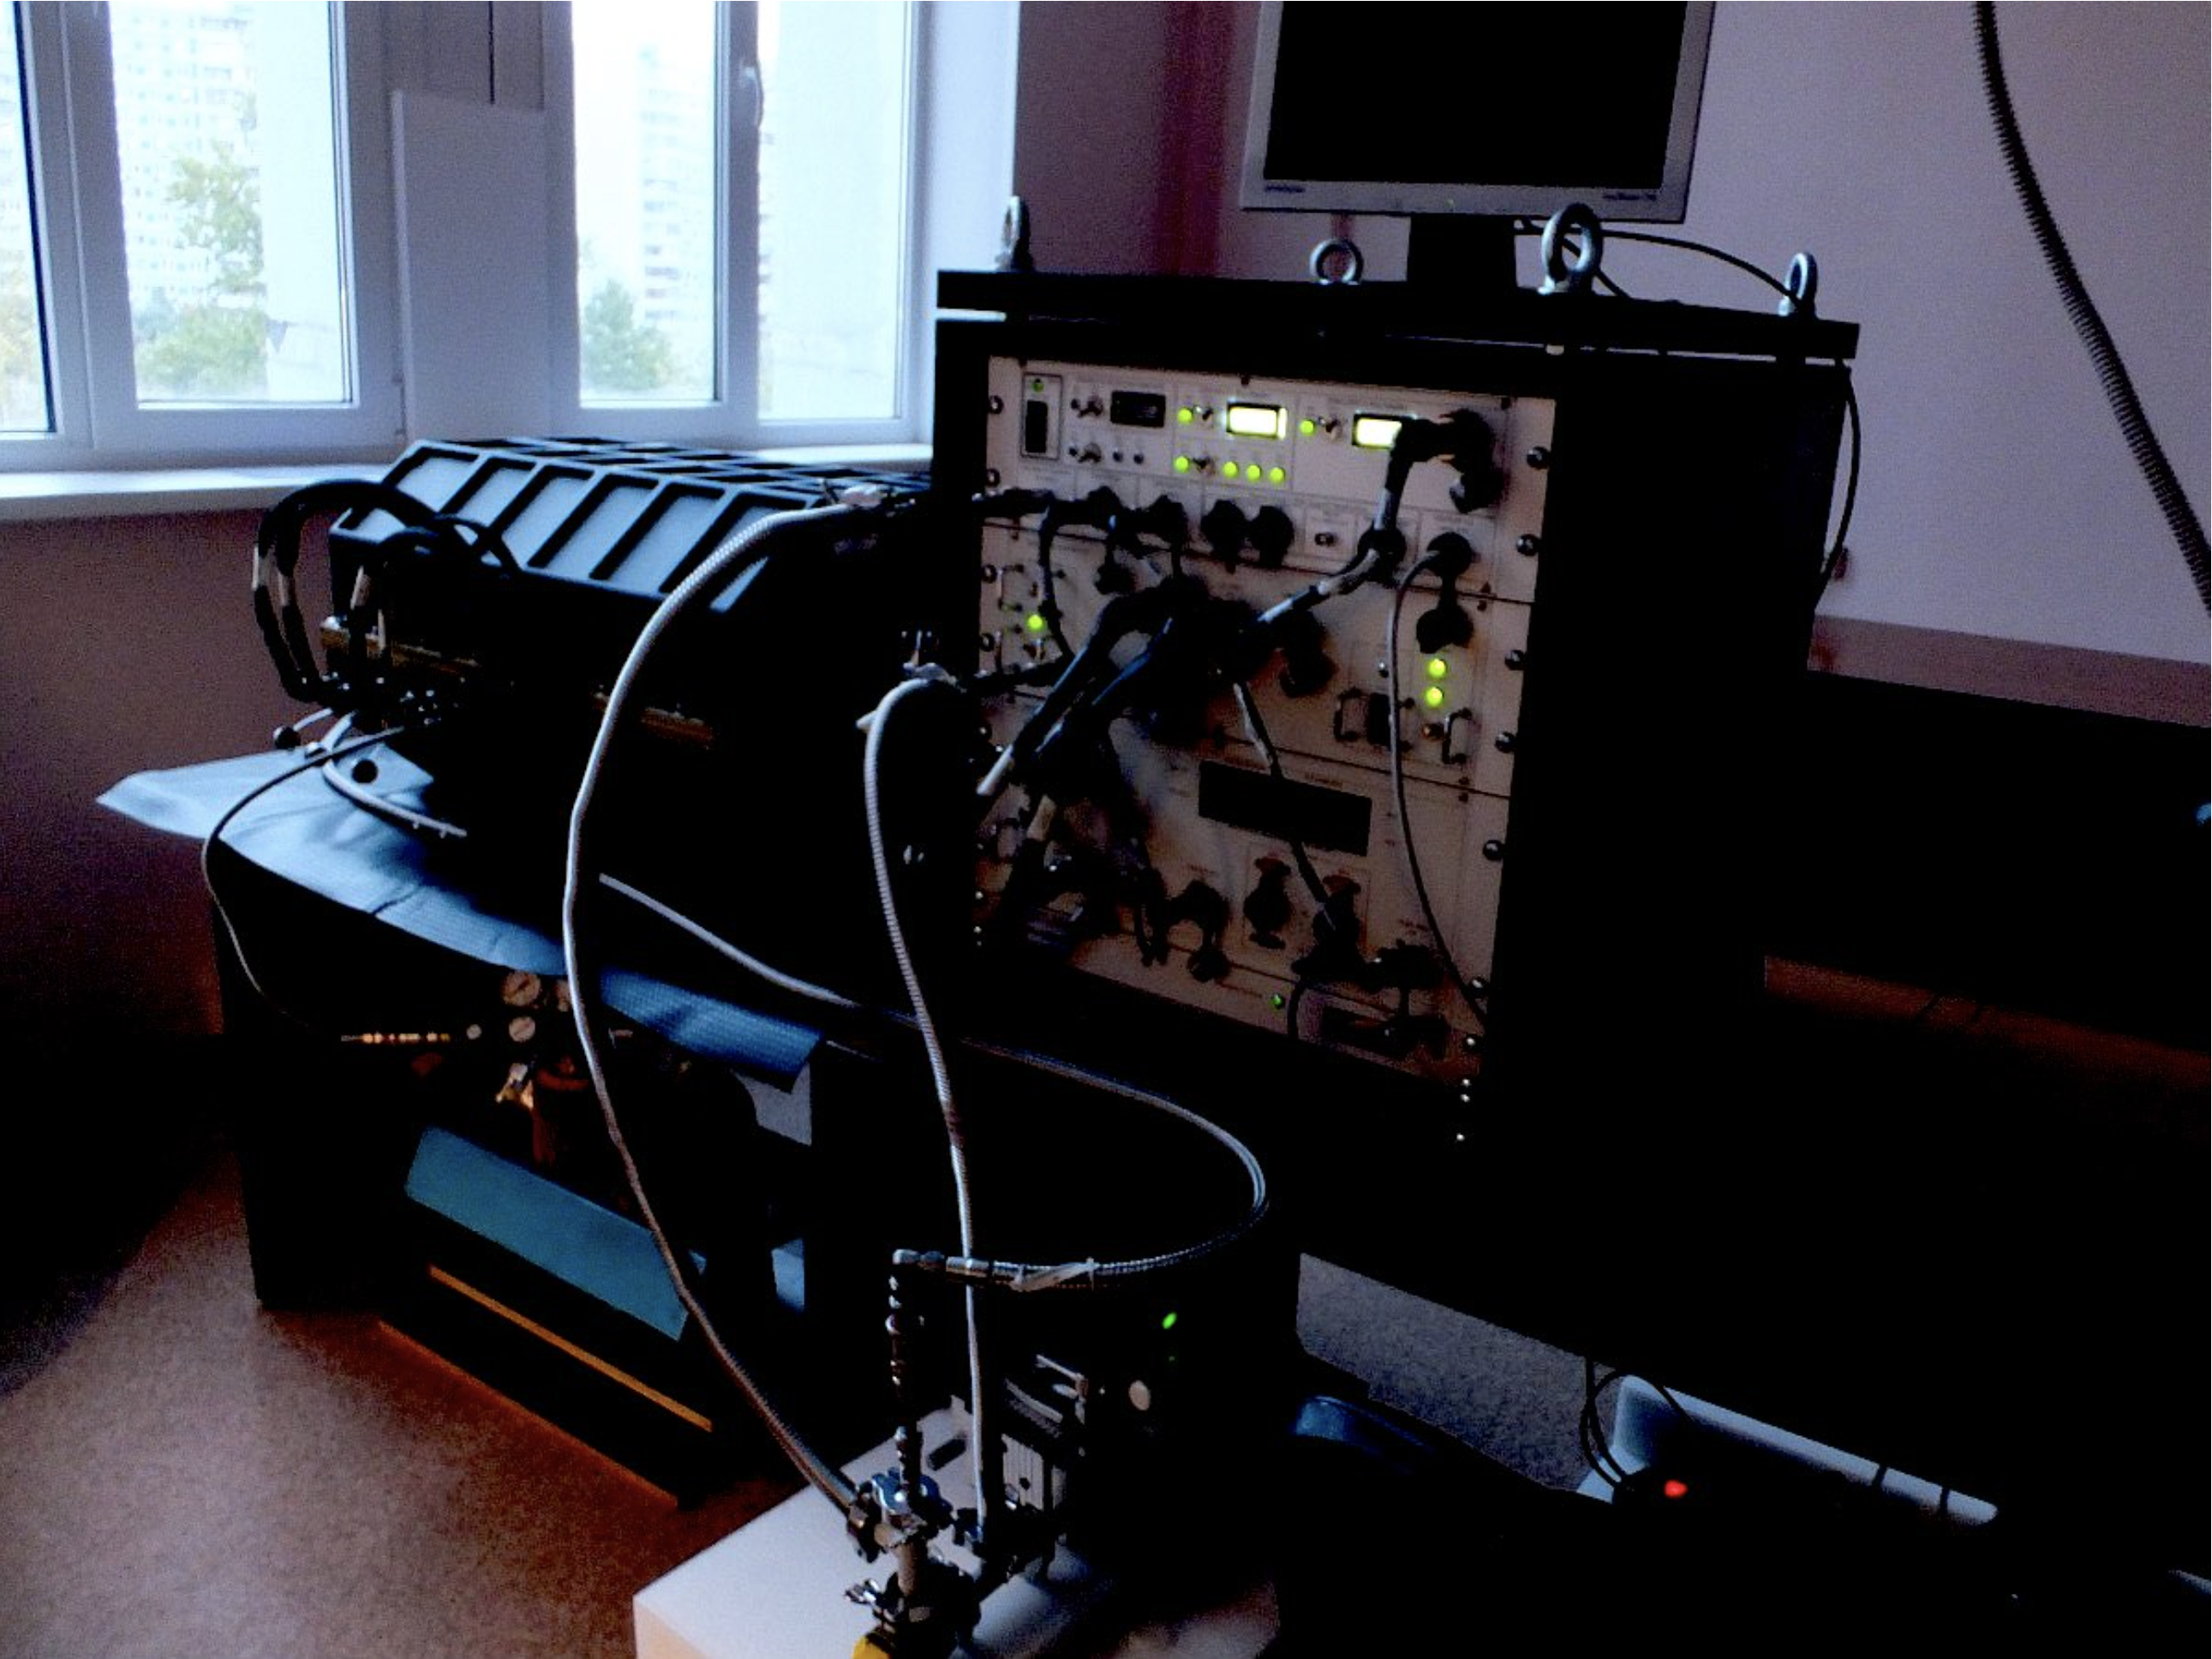
\includegraphics[width=0.5\textwidth]{figures/photo-pk4}
         }
         \caption{Экспериментальная установка научной аппаратуры «Плазменный~кристалл-4»: \pt(а) 3D-модель внутренностей,
                  \pt(б) фото уже собранной установки в лабораторных условиях.}
    \end{center}
    \label{fig:pk4}
\end{figure}

\label{sec:sec_31}
Научная аппаратура «Плазменный кристалл-4» установлена в стандартную стойку европейского лабораторного модуля «Колумбс»
Международной космической станции (МКС). ОИВТ РАН является одной из организаций-поставщиков космического
эксперимента «ПК-4» (НА «ПК-4») и имеет доступ к постановке и проведению экспериментов.

Основой экспериментальной установки является П-образная стеклянная разрядная трубка с внутренним диаметром 30~мм
и общей длиной 85~см, которая заполнена атомарным неоном под давлением 60~Па.
На концах трубки установлены цилиндрические электроды из нержавеющей стали, которые используются для создания
и поддержания разряда постоянного тока. Системы вакуумной откачки и накачки газа соединяются с концами трубки
через данные электроды. Пылевые частицы подсвечиваются зеленым (532~нм) лазерным «ножом» и
регистрируются двумя камерами наблюдения высокого разрешения (CCD1 и CCD2).
Для отслеживания макро поведения подсвеченной плазмы используется общая камера наблюдения (CCD3) (см~рис.~\ref{fig:fig31}).

Каждая камера CCD1/CCD2 имеет поле зрения \math{22 × 17}$~мм\math{^2}$, разрешение \math{1600 × 1200}$~пикселей, а также
частоту кадросмен 35~кадров в секунду. Камеры дополняют друг друга, присоединяясь меньшими сторонами и имеют общий размер
\math{44 × 17}$~мм\math{^2}$. Эффективная полуширина лазерного «ножа» составляет 50~мкм в центре поля зрения,
а также 180~мкм по краям.

Камера CCD3 имеет возможность просматривать всю трубку целиком c разрешением \math{640 × 480}$~пикселей
и частотой 15~кадров в секунду. Используя калейдоскопическую систему, камера CCD3 также наблюдает плазменное свечение
в центральной части разрядной трубки через 3~спектральных фильтра: один серый фильтр с пропусканием 12\% и два узкополосных
помеховых фильтров, настроенных на 705 и 587~нм.

Одна из копий модифицированной экспериментальной установки НА~«ПК-4«, которая в собранном виде  внешне не имеет существенных отличий,
находится в институте ОИВТ РАН (см~рис.~\ref{sub:photo-pk4}).

\section{Спектрометр «OceanOptics~USB2000+»}
Для осуществления спектральной диагностики НА~«ПК-4» применяется модульный мини-спектрометр OceanOptics~USB2000+ (см~рис.~\ref{fig:full_usb2000+}).
В основе лежит 2048-пиксельная ПЗС-линейка, которая позволяет проводить спектральные измерения в диапазоне длин
волн 350-1100~нм со спектральным разрешением 1.5~нм. Приемная головка световода спектрометра устанавливается рядом
с камерами высокого разрешения (CCD1, CCD2) и подключается к спектрометру через оптическое волокно (см~рис.~\ref{fig:fig31}).
Время считывания одного спектра составляет 4~с. Данный спектрометр также подходит для осуществления
контроля чистоты плазмы во время экспериментов.
\begin{figure}[t]
    \begin{center}
         \subfloat[\label{sub:usb2000+}]{
           \includegraphics[width=0.47\textwidth]{figures/usb2000+}
         }
         \subfloat[\label{sub:cross_section_usb2000+}]{
           \includegraphics[width=0.47\textwidth]{figures/cross_section_usb2000+}
         }
         \caption{Модульный мини-спектрометр OceanOptics~USB2000+: \pt(а) внешний вид,
                  \pt(б) внутреннее устройство.}
    \label{fig:full_usb2000+}
    \end{center}
\end{figure}

\section{Ход эксперимента}
Проведение эксперимента начинается с вакуумной откачки газоразрядной трубки. В течение 2~дней она откачивается
до давления высокого вакуума порядка \math{< 2 × 10^{-3}}$~Па, а затем заполняется неоном до рабочего давления разряда порядка 60~Па.
Ток разряда при этом составляет \math{I_{DC} = 1}$~мА. После заполнения рабочим газом, с катодной стороны разрядной
\begin{figure}[t]
  \centering
  \includegraphics[width=14cm]{figures/common_camera}
  \caption{Кадр видеозаписи с общей камеры наблюдения в ходе эксперимента, отмеченная область пылевого облака явлется областью видимости
  камер высокого разрешения (CCD1, CCD2.}
  \label{fig:common_camera}
\end{figure}
трубки с помощью пылевого инжектора впрыскиваются монодисперсные пластические (меламиноформальдегидные) микросферы
(частицы пыли) с диаметром \marh{d~=~3.38 ± 0.07}~мкм. В силу высокой подвижности электронов пылевые частицы заряжаются
отрицательно и начинают оседать на стенках трубки. Для того, чтобы поддерживать баланс гибели и рождения и плавно
управлять положением пылевого облака, необходимо регулировать электрическое поле постоянного тока с помощью напряжения
между катодом и анодом. Наблюдая за пылевым облаком через общую камеру наблюдения CCD3,
облако переносится в центр трубки (см~рис.~\ref{fig:common_camera}), где за пылевыми частицами можно наблюдать с помощью
камер высокого разрешения CCD1 и CCD2, а также осуществлять спектральную диагностику излучения.

\begin{figure}[t]
  \centering
  \includegraphics[width=16cm]{figures/high_resolution_cameras}
  \caption{Кадры видеозаписей с двух камер наблюдения высокого разрешения PGO. Кадры синхронизированы во времени, а также пространственно дополняют друг друга.}
  \label{fig:high_resolution_cameras}
\end{figure}

Таким образом, для получения эксперимента с исследуемым эффектом необходимо задать медленное движение пылевого облака при
неизменном токе между катодом и анодом, а затем провести спектральную диагностику в следующих состояниях облака:
\begin{itemize}
\item пылевое облако еще не влетело в область спектральной диагностики;
\item центр пылевого облака находится в области спектральной диагностики, что детектируется на спектре насыщенной
линией 532~нм зеленого лазера, а также видеозаписями с сопоставлением времени измерения спектров;
\item край пылевого облака попадает в область спектральной диагностики;
\end{itemize}

Поскольку облако представляет собой вытянутую овальную структуру, то можно измерить ширину облака в области спектральной диагностики
и оценить зависимость отношения интенсивностей от ширины облака, что описано в главе 4. А сейчас рассмотрим какие данные
в сыром виде приходят с НА~«ПК-4».

\section{Экспериментальные данные}
\label{cha:ch_3_4}
В научной аппаратуре «Плазменный~кристалл-4» выделены следующие каналы получения экспериментальных данных,
которые были задействованы в какой-либо мере в данной работе:
\begin{enumerate}
    \item Видеозаписи с двух камер высокого разрешения CCD1 и CCD2 (см~рис.~\ref{fig:high_resolution_cameras}).
    Видеофайлы в сыром виде имеют формат «.avi» с размером 4~Gb/min от одной камеры. На данных записях хорошо
    различимы отдельные пылевые частицы, что позволяет отслеживать их траектории движения, а также наблюдать за
    их поведением в любой момент времени.

    \item Видеозаписи с общей камеры наблюдения. Представляют собой файлы в формате «.avi» с размером 0.3~Gb/min (см~рис.~\ref{fig:common_camera}).
    На этих видеозаписях видно трубку целиком вместе с подсвеченной пылевой плазмой, где можно отследить макро поведение
    облака, в отличие от камер CCD1 и CCD2.

    \begin{figure}[t]
      \centering
      \includegraphics[width=16cm]{figures/raw_spectrum}
      \caption{Один из необработанных спектров эксперимента, полученных в ходе спектральной диагностики пылевого облака на НА~«ПК-4».}
      \label{fig:raw_spectrum}
    \end{figure}

    \item Спектральные данные. Представляют собой текстовые файлы в формате «.dat», которые имеют свою особую структуру
    по блокам, удобную для парсинга. Пример блока можно найти в \hyperref[app:app1]{приложении~А}. Эти спектральные данные
    хранят информацию о состоянии спектрометра в любой момент времени, его манипуляции, а также сырые данные с его ПЗС-линейки (см~рис.~\ref{fig:raw_spectrum}).

    \item Логи. Представляют собой текстовые файлы в формате «.log», которые содержат информацию обо всех
    технических изменениях в ходе эксперимента с временными отметками. Пример также можно найти в \hyperref[app:app2]{приложении~Б}.
\end{enumerate}

\chapter{Программа “Spectral Analyzer PK-4”}
\label{cha:ch_4}
\section{Актуальность программы}
В ходе данной работы был создан веб-сервис “Spectral~Analyzer~PK-4”, название которого состоит из двух частей:
первая часть (“Spectral~Analyzer”) обозначает главную задачу сервиса - спектральный анализ, а вторая часть говорит
о том, что анализ осуществляется на данных, полученных с исследуемой в текущей работе экспериментальной установки
“Плазменный~кристалл-4” (PK-4). Какие задачи решает “Spectral~Analyzer~PK-4”?

Наиболее важная задача - это, собственно, обработка огромного количества спектральной информации, поступающей с борта МКС
Российско-европейской Космической Аппаратуры “Плазменный~кристалл-4”. Поскольку спектральные данные представляют собой
довольно сложную, но упорядоченную структуру данных (см раздел \ref{cha:ch_3_4}), то ручная обработка и
графическое построение даже одного спектра является времязатратной и трудоёмкой задачей: необходимо ориентироваться
в текстовых логах, а также владеть навыками работы, как минимум, с двумя программами одновременно~-~Origin и Exсel.
У умелого пользователя данных программ (при большом желании) получится построить один спектр не быстрее, чем за 5~мин.
Так как в одном эксперименте возможность встретить более 1000~спектров - обычное явление, то даже таких умений становится недостаточно.

Далее, ожидается, что веб-сервис даст инструмент первичной спектральной обработки: полиномиальная калибровка длин волн,
вычитание и усреднение шумового фона, автоопределение пиков спектральных линий, усреднение идентичных спектров при одних
и тех же параметрах и др.

Мотивационный момент, в будущем данный веб-сервис может быть полезен для подготовки датасетов для применения алгоритмов
машинного обучения.

Поскольку в данной работе разработана и применена методика поиска относительного изменения электронной температуры на основе
отношения интенсивностей спектральных линий, то для “Spectral~Analyzer~PK-4” ставится задача рассчета отношений интенсивностей
спектральных линий в зависимости от энергии верхнего уровня.

Еще один мотивационный момент, данный веб-сервис потенциально дает возможность взаимодействовать
с немецкими коллегами по космической аппаратуре ПК-4.

Таким образом, было решено создать автоматизированное компьютеризированное программное обеспечение для решения данных проблем.

\section{Требования к программе}
Чтобы было не только удобно и практично пользоваться и совершенствовать программу, но и для достижения решения
поставленных задач, были выдвинуты определенные требования к программе.

Во первых, программа должна обладать свойством кроссплатформенности, т.е. независимо от типа операционной
системы она должна работать корректно. Конкретнее, должна быть возможность работы под следующими операционными
системами: Windows~XP - Windows~10, MacOs, Linux с графической оболочкой.

Во вторых, программа должна иметь возможность сохранения ключевых состояний процесса обработки данных,
а также максимально безболезненно передавать прогресс между пользователями.

Далее, программа должна уметь в автоматическом режиме загружать и парсить текстовые спектральные данные
(эксперименты), а также отображать список уже загруженных экспериментов.

Следующий важнейший аспект - это умение динамически отображать более 1000~спектральных графиков в одном
рабочем окне, отображать метаинформацию по текущему спектру.

Для обработки спектров необходимо учитывать фоновое излучение, поэтому программа должна иметь возможность по
выбранным пользователем номерам спектров усреднять их интенсивности, а также вычитать из всех спектров текущего эксперимента.

Не менее важный аспект - это возможность настроить калибровку спектра по длине волны на основе вводимой пользователем полиномиальной функции.

Далее, для поиска отношений интенсивностей необходимо на основе откалиброванных незашумленных спектров сохранять
усредненные спектры-заготовки с учётом среднеквадратичных погрешностей, также необходимо отображать
список уже сохранённых усредненных спектров.

В силу того, что используемый спектрометр “OceanOptics~USB2000+” имеет невысокую разрешающую
способность (см раздел \ref{cha:ch_3_4}), то для корректного поиска отношений интенсивностей
необходимо учитывать наложения линий друг на друга с помощью аппаратной функции спектрометра,
т.е. следующее требование к программе: она должна уметь на основе полиномиального приближения аппаратной
функции учитывать перекрытия рядом стоящих линий с учетом погрешностей.

В данной работе особый интерес представляет зависимость отношения интенсивностей определенных линий от энергии
возбужденного состояния, для этого программа должна иметь библиотеку спектральных линий, а также функционал
по выбору набора линий при построении данной зависимости.

Таким образом, мы перечислили основные требования к программе, а сейчас разберем стек технологий,
который был изучен для достижения данных целей (см.~рис.~\ref{fig:it_tech}).
\begin{figure}[t]
  \centering
  \includegraphics[width=12cm]{figures/it_tech}
  \caption{Изображены логотипы изученных IT-технологий, которые использовались для создания веб-сервиса “Spectral~Analyzer~PK-4”}
  \label{fig:it_tech}
\end{figure}

\section{Стек изученных технологий}
Первый прототип программы был написан традиционным образом на языке C\#, который непременно предполагает
стандартную установку под Windows и работу с программой, как с ПО для данной операционной системы.
В данном варианте было реализовано лишь около 20\% необходимого функционала, но при этом возникли большие трудности
с передачей программы научному руководителю из-за несовместимости версий Windows~7 и XP.

Для решения проблем кроссплатформенности и передачи данных между пользователями было решено создать веб-сервис,
который работает в обычном браузере, поскольку почти каждая операционная система с графической оболочкой
поддерживает большинство современных браузеров.

Django (Джанго)~--~свободный фреймворк для веб-приложений на языке Python, использующий шаблон проектирования MVC.
Проект поддерживается организацией Django Software Foundation \cite{Django}. Джанго имеет удобную гибкую
внутреннюю архитектуру, которая позволяет разработчикам, при достаточных знаниях, выполнять огромный спектр задач
из области веб-программирования. Перечислять все возможности данного фреймворка нет необходимости, подчеркнем лишь те,
что были использованы для решения поставленных задач.

Джанго имеет свою стандартизированную ORM, которая поддерживает транзакции. ORM (англ. Object-Relational Mapping,
рус. объектно-реляционное отображение или преобразование)~--~это некая оболочка над базой данных, которая позволяет
использовать функционал базы данных с помощью объектно-ориентированного языка программирования, в данном случае с помощью Python.

Далее, в Джанго есть система маршрутизации урлов, которая позволяет настраивать POST и GET запросы на основе регулярных выражений,
что очень удобно: в Python есть хорошо известный и понятный встроенный модуль “re”, который почти ничем не отличается по синтаксису.

В Джанго предусмотрена возможность применения криптографически шифрованных Cookie и CSRF-токенов для защиты POST
запросов к серверу: например, для аутентификации пользователя, для любого изменения и некоторых запросов к информации сервера.
Это дает довольно хорошую защиту от мошеннических и хакерских атак.

PostgreSQL~--~свободная объектно-реляционная система управления базами данных, разработанная в Калифорнийском
университете на факультете компьютерных наук в Беркли \cite{PostgreSQL}. PostgreSQL поддерживает большой набор встроенных типов данных:
\begin{itemize}
\item численные типы;
\item двоичные типы;
\item типы «дата/время»;
\item булев тип;
\item перечисление;
\item геометрические примитивы;
\item UUID-идентификатор;
\item XML-данные;
\item массивы;
\item JSON;
\item идентификаторы объектов БД;
\item псевдотипы;
\end{itemize}

NumPy является основным пакетом для научных вычислений в Python, которая поддерживает
многомерные массивы (в~т.ч.~матрицы), а также предоставляет прекрасно оптимизированные высокоуровневые методы для работы с ними,
включая математические, логические, манипуляции с размерностью, сортировку, отбор, ввод-вывод, дискретные преобразования Фурье,
основную линейную алгебру, основные статистические операции, случайное моделирование и многое другое \cite{Numpy}.
Исходный код NumPy находится в открытом доступе.

SciPy — библиотека для языка программирования Python с открытым исходным кодом, предназначенная для выполнения научных и
инженерных расчётов \cite{Scipy}. Возможности:
\begin{itemize}
\item поиск минимумов и максимумов функций;
\item вычисление интегралов функций;
\item поддержка специальных функций;
\item обработка сигналов;
\item обработка изображений;
\item работа с генетическими алгоритмами;
\item решение обыкновенных дифференциальных уравнений;
\end{itemize}

CanvasJS - библиотека для языка программирования JavaScript, которая предоставляет API для работы с диаграммами и графиками
в веб-проектах. Для студентов и некоммерческого использования лицензия предоставляется бесплатно. Основные преимущества:
\begin{itemize}
\item простой API;
\item высокая производительность;
\item 30 типов диаграмм;
\item хорошая документация;
\item поддержка браузеров Chrome, Firefox, Safari, IE8+;
\end{itemize}

При создании веб-сервиса "Spectral~Analyzer~PK-4" использовались следующие версии библиотек:
\begin{itemize}
\item django==2.0;
\item psycopg2==2.7.1;
\item numpy==1.14.2;
\item django-debug-toolbar==1.8;
\item scipy==1.0.1;
\item python-dateutil==2.6.1;
\item canvas-js==2.1
\end{itemize}

\section{Описание функционала}


\chapter{Анализ спектральных данных}
\label{cha:ch_5}

В качестве исследования были обработаны сырые спектральные данные, полученные при одних и тех же
технических условиях системы, в отсутствие пылевого облака, а также в присутствии пылевого облака (см~рис.~\ref{fig:fig34}).

\begin{figure}[t]
    \centering
    \includegraphics[width=16cm]{figures/fig34}
    \caption{
        Зависимость интенсивности (усл.~ед.) от длины волны (нм). На графике наложены три спектра:
        1. Ниже нуля калибровочный спектр с достоверными линиями неона;
        2. Жирной линией выделен спектр без пылевого облака.
        3. Тонкой линией выделен спектр с пылевым облаком
    }
    \label{fig:fig34}
\end{figure}


Экспериментально было обнаружено увеличение интенсивности спектральных линий при попадании пылевого облака
в газовый разряд неона, причем линии с разными верхними энергетическими уровнями имеют разные значения
отношений интенсивностей (см~рис.~\ref{fig:fig35}).
\begin{figure}[t]
    \centering
    \includegraphics[width=16cm]{figures/fig35}
    \caption{Зависимость отношения интенсивностей спектральных линий неона в присутствии пылевого облака к отсутствию пылевого облака.}
    \label{fig:fig35}
\end{figure}


% [МОЖЕТ СТОИТ ВЫНЕСТИ ДАЛЬНЕЙШИЕ РАССУЖДЕНИЯ В РАЗДЕЛ "АНАЛИЗ СПЕКТРАЛЬНЫХ ДАННЫХ" ???]

Поскольку электроны, имеющие энергию выше пороговой участвуют в неупругих столкновениях с атомами, то ФРЭ должно иметь
двухтемпературное распределение [ССЫЛКА???]. Несложно заметить, что полученные расчетные ФРЭ также имеют двухтемпературный вид:
на рис. {\ref{sub:log_fre_start}} распределения можно аппроксимировать прямыми линиями со своими электронными
температурами, но хвостовые части (см.~рис.~\ref{sub:log_fre_tail}) идеально описываются прямыми линиями. Запишем распределение хвостовой части ФРЭ:
\begin{equation}
    f_{tail}(\epsilon) = e^{-{\epsilon \over T_e}} \Rightarrow ln(f_{tail}) = - {\epsilon \over T_e}.
    \label{eq:tail}
\end{equation}

В рамках одного и того же переходного процесса справедливы следующие рассуждения: интенсивность
спектральной линии пропорциональна заселенности верхнего уровня данного перехода, которая в свою очередь
пропорциональна скорости заселения верхнего уровня, т.е.:
\begin{equation}
I(T_e) \sim N^*(T_e) \sim X_{exc}(T_e).  % \sim  \int_{E_{th}}^{\infty} \sigma(\epsilon)f_{tail}(\epsilon)\sqrt{\epsilon}d\epsilon
\label{eq:sim_Te}
\end{equation}

Скорость заселения верхних уровней определяется следующим выражением [МОЖЕТ СТОИТ ВЫНЕСТИ ЕГО В РАЗДЕЛ 1.1 ???]:
\begin{equation}
    X_{exc} (T_e) = \sqrt{2 \over m} \int_{E_{th}}^{\infty} \sigma(\epsilon)f(\epsilon)\sqrt{\epsilon}d\epsilon,
    \label{eq:velocity}
\end{equation}
где \math{\sigma (\epsilon)}$~--~сечение неупругих столкновений для переходного уровня в зависимости от энергии;
\math{f (\epsilon)}$~--~ФРЭ.

Используя выражения (\ref{eq:sim_Te}) и (\ref{eq:velocity}) для двух различных конфигураций газового разряда и выбранной
спектральной линии в рамках одного переходного процесса, имеем:
\begin{equation}
{{I_2} \over {I_1}}= {{\int_{E_{th}}^{\infty} \sigma(\epsilon)f_{2}(\epsilon)\sqrt{\epsilon}d\epsilon} \over
{\int_{E_{th}}^{\infty} \sigma(\epsilon)f_{1}(\epsilon)\sqrt{\epsilon}d\epsilon}},
\label{eq:intensities_ratio}
\end{equation}
где индексы 1 и 2 обозначают различные конфигурации самосогласованного газового разряда, т.е. при различных осевых
электрических полях. Сечение \math{\sigma}$ и пороговая энергия \math{E_{th}}$ не различаются для двух конфигураций.
Следует отметить, что энергия верхнего уровня влияет на значение отношения интенсивностей, что мы и наблюдаем в эксперименте (см.~рис~\ref{fig:fig16}).

Таким образом, выполнив перебор всех расчетных ФРЭ для различных осевых электрических, можно понять по отношению
интенсивностей спектральных линий и (\ref{eq:intensities_ratio}), какая из ФРЭ описывает новую конфигурацию
газового разряда. Затем по хвостовой части ФРЭ из (\ref{eq:tail}) несложно вычислить и электронную температуру:
\begin{equation}
    T_{e,2} = {ln(f_{tail,1}) \over ln(f_{tail,2})} T_{e,1}.
\end{equation}

% ПЕРЕНЕСТИ
\begin{figure}[t]
  \centering
  \includegraphics[width=16cm]{figures/fig16}
  \caption{Зависимость ...... .}
  \label{fig:fig16}
\end{figure}


\backmatter %% Здесь заканчивается нумерованная часть документа и начинаются ссылки и
            %% заключение

\Conclusion % заключение к отчёту

В ходе решения поставленной задачи была разработана методика определения относительного изменения электронной
температуры по эмиссионным спектрам в положительном столе газового разряда постоянного тока, которая показала
достаточно хорошую согласованность с экспериментом. Проведена спектральная диагностика данного газового разряда
в возмущенном и невозмущенном пылевым облаком состояниях, в ходе которой наблюдался неравномерный рост интенсивностей
спектральных линий для различных возбужденных состояний. Данный эффект в космических условиях выражен сильнее, чем
в условиях земной гравитации. Оценены абсолютные значения электронной температуры и осевого электрического поля
для возмущенного пылевыми частицами газового разряда на основе параметров невозмущенного разряда
по эмиссионным спектрам, что не было сделано ранее. Реализован веб-сервис «Spectral~Analyzer~PK-4», который
используется для обработки огромного числа спектральных данных, полученных с научной аппаратуры
«Плазменный~кристалл~-~4».



\include{51-biblio}

\appendix   % Тут идут приложения

\App
\label{app}

\section{Приложение А}
\label{app:app1}
Пример записи блока (одного спектра) в эксперименте. Спектральный файл обычно содержит более 1000 таких блоков, которые
следуют друг за другом.

\begin{small}
\begin{verbatim}
###############################################################################
# PK4 EAC SW -- Spectrometer
# started   2016-10-12'13:57:45.58 ~
# HPC=7679703032397 / HPCFreq=1496280000 Hz => HPC uptime = 5132.530698 s
# 2016-10-12'13:57:42.55; spectrometer commanded
# 2016-10-12'13:57:45.58; spectrometer response received
#--- spectrum ---
# 65535; spectrum start marker
#     0; data size flag
#     1; nr scans accumulated
#   750; integration time /ms
#     0; reserved value FPGA_ESV_MSW
# 12118; reserved value FPGA_ESV_LSW
#     0; pixel mode
   0:     0
   1:   471
   2:   484
   3:   466
   4:   510
   5:   506
   6:   484
   7:   451
   8:   491
   9:  1729
………..
1022:   537
1023:   623
1024:   557
1025:   493
1026:   525
………..
2038:   506
2039:   578
2040:   585
2041:   548
2042:   618
2043:   546
2044:   650
2045:   549
2046:   541
2047:   516
# 65533; spectrum end marker
#=== spectrum === read-out time = 2.172 s
# ended     2016-10-12'13:57:45.63 ~ (execution time = 0.051892 s)
# PK4 EAC SW -- Spectrometer
###############################################################################
\end{verbatim}
\end{small}

\section{Приложение Б}
\label{app:app2}

\end{document}
